\begin{figure}[t]
\centering
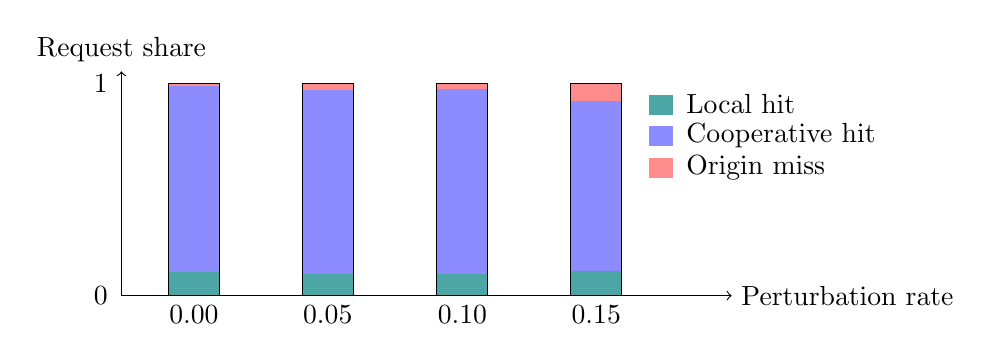
\begin{tikzpicture}[x=1cm,y=1cm]
\draw[->] (0.55,0.45) -- (8.30,0.45) node[right] {Perturbation rate};
\draw[->] (0.55,0.45) -- (0.55,3.30) node[above] {Request share};
\node[left] at (0.50,0.45) {0};
\node[left] at (0.50,3.15) {1};
\fill[teal!70] (1.15,0.45) rectangle (1.80,0.75);
\fill[blue!45] (1.15,0.75) rectangle (1.80,3.11);
\fill[red!45] (1.15,3.11) rectangle (1.80,3.15);
\draw (1.15,0.45) rectangle (1.80,3.15);
\node[below] at (1.47,0.45) {0.00};
\fill[teal!70] (2.85,0.45) rectangle (3.50,0.72);
\fill[blue!45] (2.85,0.72) rectangle (3.50,3.06);
\fill[red!45] (2.85,3.06) rectangle (3.50,3.15);
\draw (2.85,0.45) rectangle (3.50,3.15);
\node[below] at (3.17,0.45) {0.05};
\fill[teal!70] (4.55,0.45) rectangle (5.20,0.73);
\fill[blue!45] (4.55,0.73) rectangle (5.20,3.07);
\fill[red!45] (4.55,3.07) rectangle (5.20,3.15);
\draw (4.55,0.45) rectangle (5.20,3.15);
\node[below] at (4.88,0.45) {0.10};
\fill[teal!70] (6.25,0.45) rectangle (6.90,0.76);
\fill[blue!45] (6.25,0.76) rectangle (6.90,2.92);
\fill[red!45] (6.25,2.92) rectangle (6.90,3.15);
\draw (6.25,0.45) rectangle (6.90,3.15);
\node[below] at (6.58,0.45) {0.15};
\fill[teal!70] (7.25,2.75) rectangle (7.55,3.00); \node[right] at (7.60,2.88) {Local hit};
\fill[blue!45] (7.25,2.35) rectangle (7.55,2.60); \node[right] at (7.60,2.48) {Cooperative hit};
\fill[red!45] (7.25,1.95) rectangle (7.55,2.20); \node[right] at (7.60,2.08) {Origin miss};
\end{tikzpicture}
\caption{Hit-ratio decomposition for Adaptive TACC. Most served demand is cooperative rather than purely local, showing why graph-aware cache diversity matters.}
\label{fig:generated_hit_breakdown}
\end{figure}
